\problemname{Förvirrad föreläsare}


Bjarki undervisar på en kurs på universitetet, men är
inte särskilt organiserad av sig. Särskilt förvirrad blir han av att antalet föreläsningar
varierar från vecka till vecka.

Om kursen har $A$ schemalagda föreläsningar första veckan och $B$
föreläsningar nästa vecka, kommer Bjarki ändå bara att hålla exakt $A$ föreläsningar. Därför
kan det ibland hända att Bjarki håller lektion inför tomt klassrum och ibland att han inte dyker upp när han ska. I slutet av veckan
får han dock ett argt brev av sin chef med vilka tider han skulle hållit
föreläsningar och kommer istället att använda dessa tider veckan därpå. 

Skriv ett program som, givet antalet schemalagda föreläsningar under $N$ veckor, skriver ut antalet
föreläsningar Bjarki kommer hålla inför tomma klassrum samt antalet
föreläsningar Bjarki inte dyker upp på.

\begin{figure}[ht!]
\centering
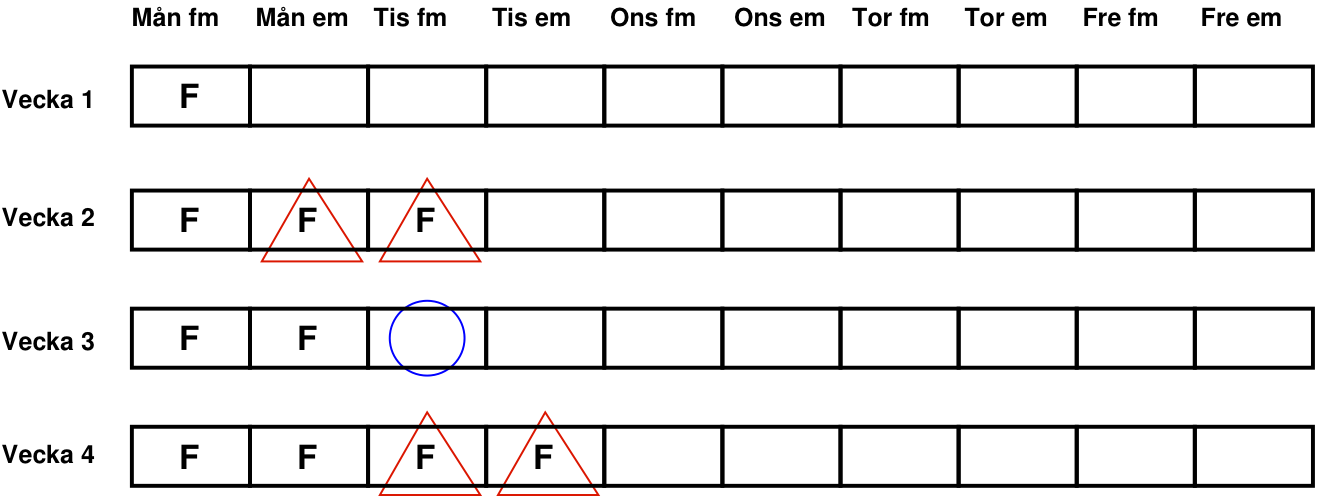
\includegraphics[width=0.8\textwidth]{forelasare.png}
\caption{Schemat i det första exemplet. F markerar schemalagda föreläsningar. En blå cirkel markerar att Bjarki håller lektionen inför tomt klassrum och en röd triangel markerar att han inte dyker upp. {\bf Förklaring:} Första veckan har Bjarki alltid koll på vilka
föreläsningar han ska hålla. Veckan därpå tror han att han bara ska
hålla en föreläsning, och missar därför två stycken. Tredje veckan håller han
tre föreläsningar, varav en inför tomt klassrum, och sista veckan missar han två
föreläsningar. Totalt har han hållt 1 tom föreläsning och missat 4 föreläsningar.} }
\label{overflow}
\end{figure}


\section*{Indata}

Först kommer talet $N$ på en egen rad, där $1\le N \le 9$. Därefter kommer $N$ heltal, antalet
schemalagda föreläsningar under var och en av veckorna.

Det kan aldrig vara mer än 10 föreläsningar under en vecka och tiderna fylls alltid på från början av veckan utan luckor (se figuren ovan). 

\section*{Utdata}
Skriv ut antalet tomma föreläsningar Bjarki har hållt, ett mellanslagtecken,
därefter antalet föreläsningar Bjarki har missat.
